\documentclass[10pt,a4paper]{article}
\usepackage[latin1]{inputenc}
\usepackage{amsmath}
\usepackage{amsfonts}
\usepackage{amssymb}
\usepackage{fullpage}
\usepackage{graphicx}

\begin{document}
\title{Goldstein, Poole, and Safko Problem 3.32}
\author{Josh Orndorff \\ admin@joshorndorff.com}
\maketitle

\section{The Geometric Optics Problem}
Our convention for angles is that the angles of incidence and refraction, $\theta_1$, $\theta_2$, and $\theta_3$ are positive definite, while the angles, $\phi$, and $\Theta$ are positive if they are counter clockwise from the blue diameter and negative otherwise.  In the particular figure, both $\phi$ and $\Theta$ are negative.

\begin{figure}
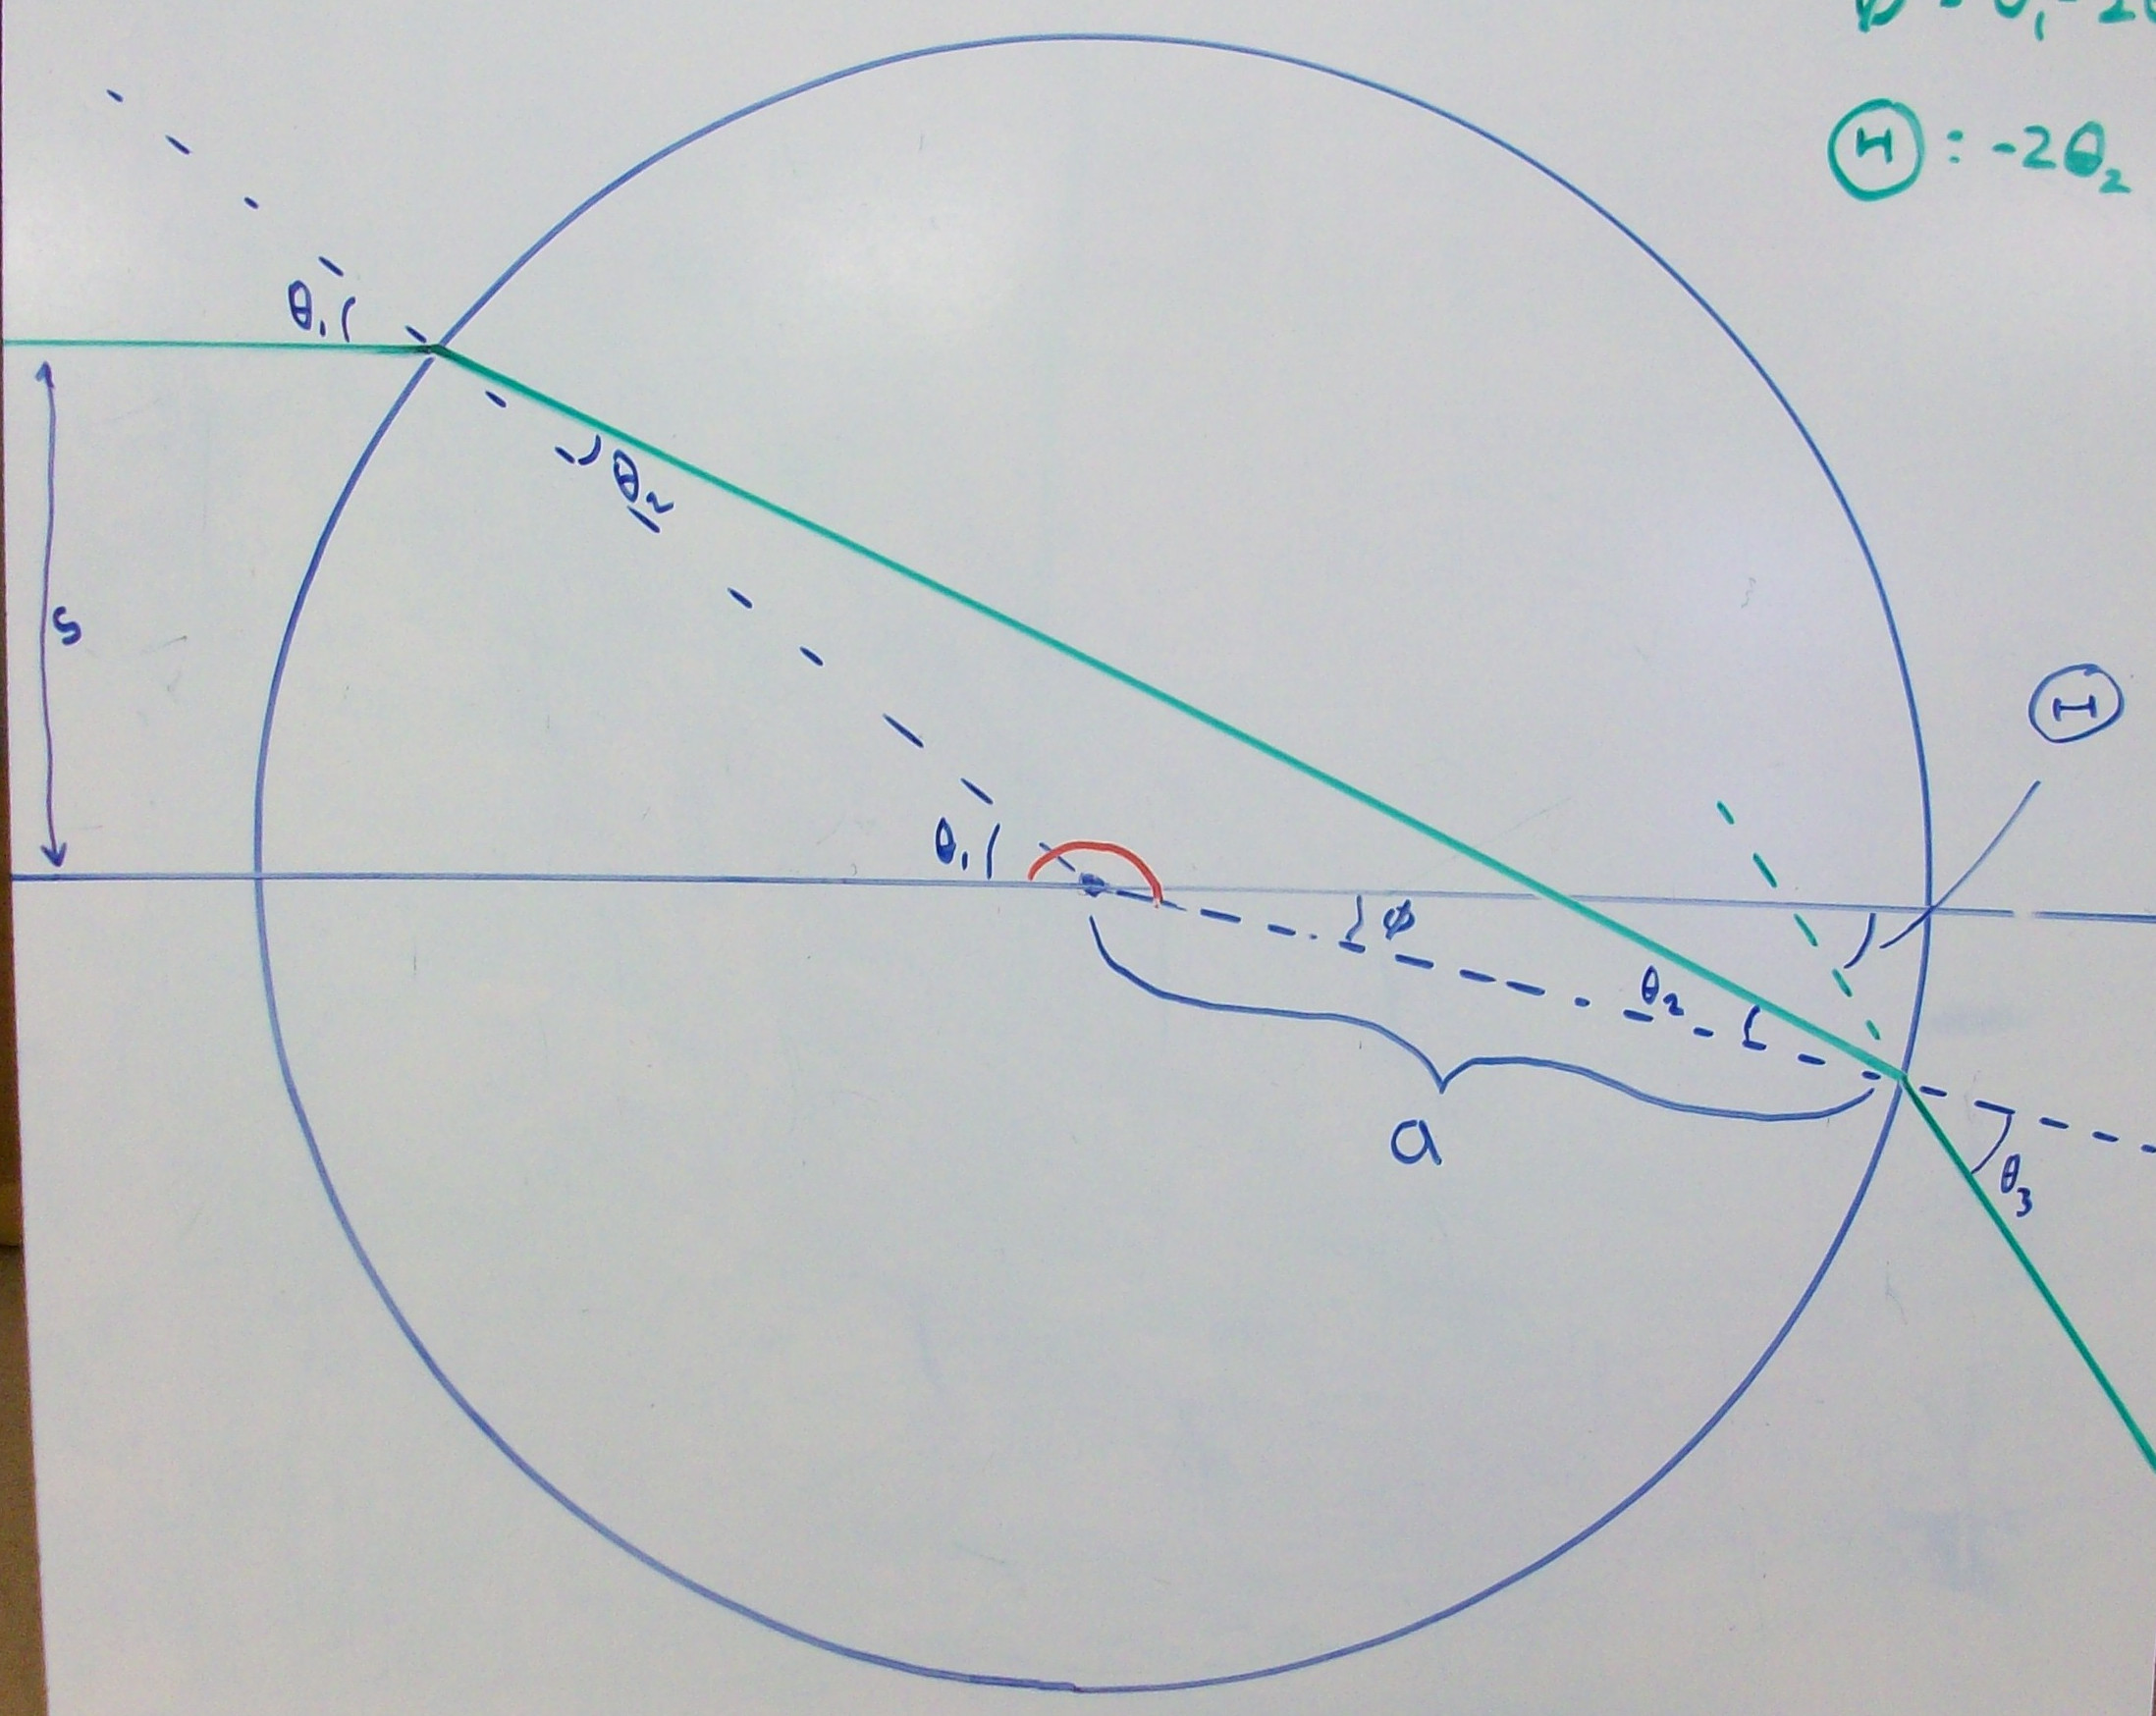
\includegraphics[scale=1]{Goldstein3-32.jpg}
\end{figure}

We'll start by finding an expression for $\theta_1$.
\begin{equation}
\sin\theta_1=\frac{s}{a}
\end{equation}

Using Snell's law we can find $\theta_2$.
\begin{equation}
\sin\theta_2=\frac{\sin\theta_1}{n}=\frac{s}{na}
\end{equation}

And using Snell's law again, we can find $\theta_3$.
\begin{equation}
\sin\theta_3=n\sin\theta2
\end{equation}
Plugging in the form of $\theta_2$ that we found previously, we get the following.
\begin{equation}
\sin\theta_3=n\frac{\sin\theta_1}{n}=\sin\theta_1
\end{equation}

So we see that $\theta_3 = \theta_1$.  We get this result without any assumptions of the ray's incident location on the sphere.  Now we need to find the scattering angle $\Theta$.  It should be evident from the diagram and our sign convention that $\Theta=\phi-\theta_3$.

We can find $\phi$ using some geometric observations from the diagram.  Note that the ray's path through the sphere is the base of an isosceles triangle with base angles $\theta_2$.  Therefore the top angle must be given by $180^\circ-2\theta_2$.  The entire red angle in the diagram is then given by $180^\circ-2\theta_2+\theta_1$. And finally we can get and expression for the magnitude of $\phi$.
\begin{equation}
|\phi|=180^\circ-2\theta_2+\theta_1-180^\circ=\theta_1-2\theta_2
\end{equation}
Plugging $\phi$ into $\Theta$ while remembering our sign convention and that $\theta_1=\theta_3$.
\begin{equation}
\Theta=-\theta_1+2\theta_2-\theta_3=2\theta_2-2\theta_1
\end{equation}
\begin{equation}
\Theta 2\left[\arcsin \frac{s}{na}-\arcsin\frac{s}{a}\right]
\end{equation}

\section{The Classical Mechanics Problem}


\end{document}